% Name: Riemann sum
% Description: Eight left-endpoint rectangles under a curve, approximating its integral.
% Tags: Riemann sum, integral, approximation

\usetikzlibrary{arrows.meta}

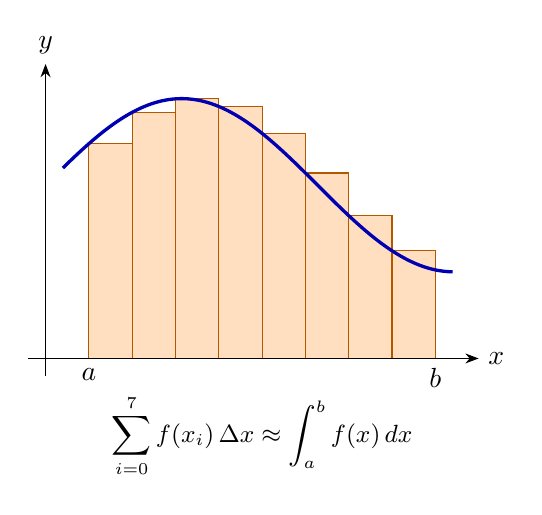
\begin{tikzpicture}[>={Stealth}, scale=1.1]
  \foreach \i in {0,...,7} {
    \pgfmathsetmacro\x{0.5 + 0.5*\i}
    \pgfmathsetmacro\h{2 + sin(deg(\x))}
    \draw[fill=orange!25, draw=orange!70!black] (\x,0) rectangle ++(0.5,\h);
  }
  \draw[->] (-0.2,0) -- (5,0) node[right] {$x$};
  \draw[->] (0,-0.2) -- (0,3.4) node[above] {$y$};
  \draw[very thick, blue!70!black, domain=0.2:4.7, samples=60, smooth]
    plot (\x, {2 + sin(deg(\x))});
  \node[below] at (0.5,0) {$a$};
  \node[below] at (4.5,0) {$b$};
  \node[font=\small, align=center] at (2.5,-0.9) {$\displaystyle\sum_{i=0}^{7} f(x_i)\,\Delta x \approx \int_a^b f(x)\,dx$};
\end{tikzpicture}
